\documentclass[11pt]{article}

\usepackage[utf8]{inputenc}
\usepackage{amsmath}
\usepackage{graphicx}
\usepackage{enumerate}
\usepackage{subcaption}
\usepackage{hyperref}
\usepackage{hypcap}
\usepackage{relsize}
\usepackage{caption}
\usepackage{array} 
\usepackage[margin=1in, paperwidth=8.5in, paperheight=11in]{geometry}
\usepackage{float}
\usepackage{array}
\usepackage{tabularx}
\usepackage{textgreek}
\usepackage{amsmath}
\usepackage{amssymb}
\usepackage{amsthm}
\usepackage{parskip}
\usepackage{svg}
\usepackage{blindtext}
\usepackage{listings}
\usepackage{xcolor}
\usepackage{siunitx}
% \hypersetup{
%     colorlinks=true,
%     linkcolor=blue,
%     filecolor=magenta,
%     urlcolor=cyan,
% }
\lstset{
  basicstyle=\ttfamily,
  columns=fullflexible,
  % frame=single,
  breaklines=true,
  postbreak=\mbox{\textcolor{red}{$\hookrightarrow$}\space},
}

\usepackage{graphicx}
\title{Miniproject 2: CSRL Shift Register}
\author{Drew Pang }
\date{6 October, 2025}

\begin{document}

\maketitle

\section*{Schematic Capture and Simulation}

\subsection*{$\phi$ and $\bar{\phi}$  CSRL Latches}

\begin{figure}[H]
  \centering
  \includesvg[inkscapelatex=false,width=8cm]{media/csrl.svg}
  \includesvg[inkscapelatex=false,width=8cm]{media/csrl_n.svg}
  \caption{$\phi$ and $\bar{\phi}$ CSRL latch transistor level schematics}
\end{figure}

\begin{figure}[H]
  \centering
  \includesvg[inkscapelatex=false,width=5cm]{media/csrl_sym.svg}
  \includesvg[inkscapelatex=false,width=5cm]{media/csrl_n_sym.svg}
  \caption{$\phi$ and $\bar{\phi}$ CSRL latch transistor level symbols}
\end{figure}

I created $\phi$ and $\bar{\phi}$ CSRL latches folowing designed outlined in \textit{Wiring Considerations in Analog VLSI Systems, with Applications to Field-Programmable Networks} by Dr. Sivilotti. I used a 4:1 ratio for transistors M14 and M4 in the $\phi$ and $\bar{\phi}$ latches respectively, based on a recommendation in the paper. Given the lower operating voltage of the Sky130A process, this ratio could certainly be optimized further. 

\subsection*{Rising Edge Triggered CSRL Latch}

\begin{figure}[H]
  \centering
  \includesvg[inkscapelatex=false,width=8cm]{media/csrl_rising_edge.svg}
  \caption{Rising edge-triggered CSRL latch schematic}
\end{figure}

\begin{figure}[H]
  \centering
  \includesvg[inkscapelatex=false,width=5cm]{media/csrl_rising_edge_sym.svg}
  \caption{Rising edge-triggered CSRL latch symbol}
\end{figure}

A rising-triggered latch can be constructed with a $\bar{\phi}$ latch followed by a $\phi$ latch.

\subsection*{Simulation and Test Harness}

\begin{figure}[H]
  \centering
  \includesvg[inkscapelatex=false,width=\linewidth]{media/csrl_rising_edge_x4_tran.svg}
  \caption{CMOS AND gate schematic and symbol}
\end{figure}

I set up a test harness with a pulse on the input to the shift register, initial conditions on intermediate and output nodes, and a specific simulation corner (i.e. TT, SS, SF, FS, FF). Transient simulation plots are shown in figures 6-9.

\begin{figure}[H]
  \centering
  \includegraphics[width=13cm]{media/csrl_rising_edge_x4_ss.png}
  \caption{Rising edge-triggered CSRL latch simulated at the SS corner}
\end{figure}

\begin{figure}[H]
  \centering
  \includegraphics[width=13cm]{media/csrl_rising_edge_x4_sf.png}
  \caption{Rising edge-triggered CSRL latch simulated at the SF corner}
\end{figure}

\begin{figure}[H]
  \centering
  \includegraphics[width=13cm]{media/csrl_rising_edge_x4_fs.png}
  \caption{Rising edge-triggered CSRL latch simulated at the FS corner}
\end{figure}

\begin{figure}[H]
  \centering
  \includegraphics[width=13cm]{media/csrl_rising_edge_x4_ff.png}
  \caption{Rising edge-triggered CSRL latch simulated at the FF corner}
\end{figure}

As seen in the simulation plots, my design is resistant to variations in the process node. Optimizing the width of the critical pull down and pull up transistors in the $\phi$ and $\bar\phi$ latches could be sped up my automating the generation and analysis of plots like those in figures 6-9.

\section*{Layout Design}

\subsection*{Rising Edge-Triggered CSRL Latch}
\begin{figure}[H]
  \centering
  \includegraphics[width=6cm]{media/rising_edge_csrl.png}
  \caption{Rising edge-triggered CSRL latch}
\end{figure}

My rising edge-triggered CSRL latch is comprised of $\phi$ and $\bar{\phi}$  CSRL latches, with the VP, D/Q, clk, Dn/Qn, and VN nets running horizontally. Excluding the extended nwell and m1, my CSRL edge-triggered latch measures 4.75x\qty{8.25}{\micro\meter}.

\subsection*{Four-Bit Shift Register}
\begin{figure}[H]
  \centering
  \includegraphics[width=\linewidth]{media/rising_edge_shift_register.png}
  \caption{Four-bit shift register comprised of four rising edge-triggered CSRL latches }
\end{figure}

I constructed a four-bit shift register by abutting four copies of my rising edge CSRL latch. The final design passes DRC and measures 18.5x\qty{8.25}{\micro\meter}

\subsection*{Falling Edge-Triggered CSRL Latch}
\begin{figure}[H]
  \centering
  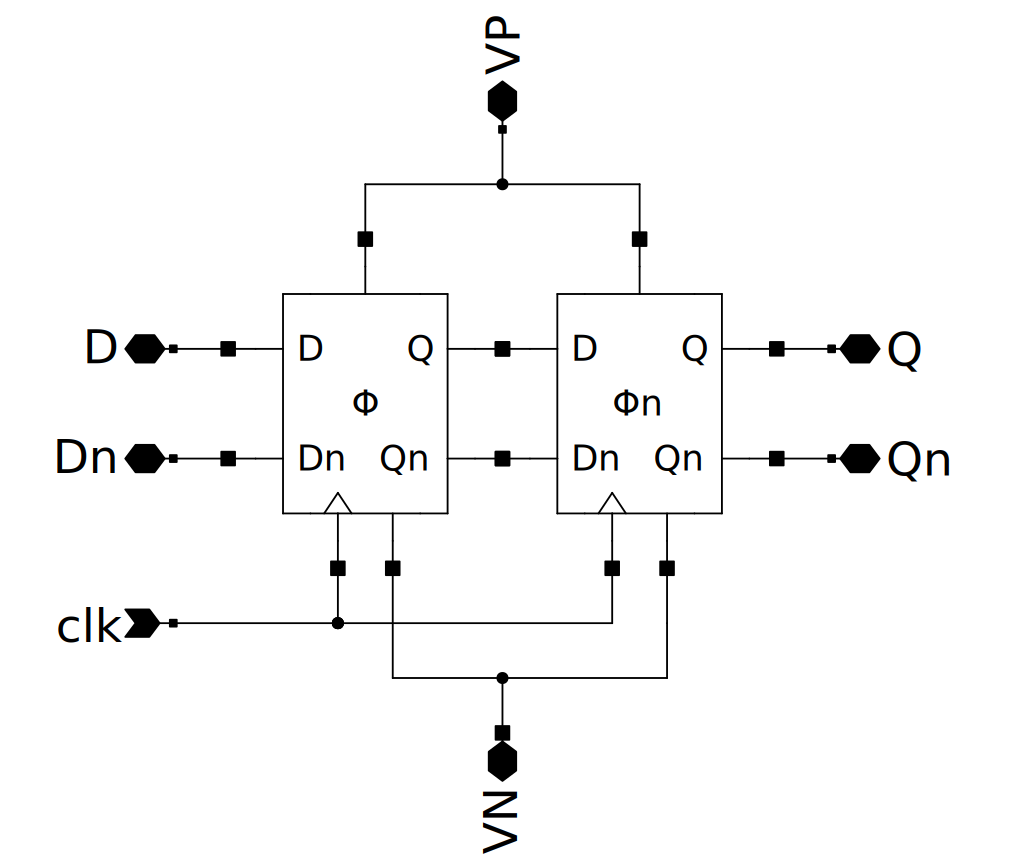
\includegraphics[width=6cm]{media/csrl_edge.png}
  \caption{Falling edge-triggered CSRL latch}
\end{figure}

\subsection*{Four-Bit Shift Register}
\begin{figure}[H]
  \centering
  \includegraphics[width=\linewidth]{media/shift_register.png}
  \caption{Four-bit shift register comprised of four falling edge-triggered CSRL latches }
\end{figure}

I mistakenly made a falling edge shift register first. It measured 18.4x\qty{8.15}{\micro\meter}.



\section*{Layout Versus Schematic}

Netcomp reported matches between my schematic and layout. The Netcomp output and log file can be found in appendix A and B respectively. One change was made to the netlist from Magic, which is show in appendix C. \\

This change was to the top level of the netlist from the layout. Whereas Xschem output a netlist with the top level hierarchy removed, Magic did not. Without this change, LVS fails due to the mismatch between the ports at the top level.




\newpage

\section*{Appendix A: Netcomp Output}
\begin{lstlisting}
Netgen 1.5.300 compiled on Sat Sep 20 09:39:56 PM EDT 2025
Warning: netgen command 'format' use fully-qualified name '::netgen::format'
Warning: netgen command 'global' use fully-qualified name '::netgen::global'
Reading netlist file shift_register.spice
Call to undefined subcircuit sky130_fd_pr__pfet_01v8
Creating placeholder cell definition.
Call to undefined subcircuit sky130_fd_pr__nfet_01v8
Creating placeholder cell definition.
Reading netlist file shift_register_xschem.spice
Call to undefined subcircuit csrl_edge
Creating placeholder cell definition.
Call to undefined subcircuit csrl
Creating placeholder cell definition.
Call to undefined subcircuit csrl_n
Creating placeholder cell definition.
Call to undefined subcircuit sky130_fd_pr__pfet_01v8
Creating placeholder cell definition.
Call to undefined subcircuit sky130_fd_pr__nfet_01v8
Creating placeholder cell definition.

Reading setup file /usr/local/share/pdk/sky130A/libs.tech/netgen/sky130A_setup.tcl

Model sky130_fd_pr__nfet_01v8 pin 1 == 3
No property mult found for device sky130_fd_pr__nfet_01v8
No property sa found for device sky130_fd_pr__nfet_01v8
No property sb found for device sky130_fd_pr__nfet_01v8
No property sd found for device sky130_fd_pr__nfet_01v8
No property nf found for device sky130_fd_pr__nfet_01v8
No property nrd found for device sky130_fd_pr__nfet_01v8
No property nrs found for device sky130_fd_pr__nfet_01v8
No property area found for device sky130_fd_pr__nfet_01v8
No property perim found for device sky130_fd_pr__nfet_01v8
No property topography found for device sky130_fd_pr__nfet_01v8
Model sky130_fd_pr__nfet_01v8 pin 1 == 3
No property area found for device sky130_fd_pr__nfet_01v8
No property perim found for device sky130_fd_pr__nfet_01v8
No property topography found for device sky130_fd_pr__nfet_01v8
Model sky130_fd_pr__pfet_01v8 pin 1 == 3
No property mult found for device sky130_fd_pr__pfet_01v8
No property sa found for device sky130_fd_pr__pfet_01v8
No property sb found for device sky130_fd_pr__pfet_01v8
No property sd found for device sky130_fd_pr__pfet_01v8
No property nf found for device sky130_fd_pr__pfet_01v8
No property nrd found for device sky130_fd_pr__pfet_01v8
No property nrs found for device sky130_fd_pr__pfet_01v8
No property area found for device sky130_fd_pr__pfet_01v8
No property perim found for device sky130_fd_pr__pfet_01v8
No property topography found for device sky130_fd_pr__pfet_01v8
Model sky130_fd_pr__pfet_01v8 pin 1 == 3
No property area found for device sky130_fd_pr__pfet_01v8
No property perim found for device sky130_fd_pr__pfet_01v8
No property topography found for device sky130_fd_pr__pfet_01v8
Comparison output logged to file comp.out
Logging to file "comp.out" enabled
Circuit sky130_fd_pr__pfet_01v8 contains no devices.
Circuit sky130_fd_pr__nfet_01v8 contains no devices.

Contents of circuit 1:  Circuit: 'csrl_edge'
Circuit csrl_edge contains 14 device instances.
  Class: sky130_fd_pr__nfet_01v8 instances:   7
  Class: sky130_fd_pr__pfet_01v8 instances:   7
Circuit contains 11 nets.
Contents of circuit 2:  Circuit: 'csrl_edge'
Circuit csrl_edge contains 14 device instances.
  Class: sky130_fd_pr__nfet_01v8 instances:   7
  Class: sky130_fd_pr__pfet_01v8 instances:   7
Circuit contains 11 nets.

Circuit 1 contains 14 devices, Circuit 2 contains 14 devices.
Circuit 1 contains 11 nets,    Circuit 2 contains 11 nets.


Contents of circuit 1:  Circuit: 'shift_register.spice'
Circuit shift_register.spice contains 4 device instances.
  Class: csrl_edge             instances:   4
Circuit contains 13 nets.
Contents of circuit 2:  Circuit: 'shift_register_xschem.spice'
Circuit shift_register_xschem.spice contains 4 device instances.
  Class: csrl_edge             instances:   4
Circuit contains 13 nets.

Circuit 1 contains 4 devices, Circuit 2 contains 4 devices.
Circuit 1 contains 13 nets,    Circuit 2 contains 13 nets.


Final result: 
Circuits match uniquely.
.
Logging to file "comp.out" disabled
LVS Done.
\end{lstlisting}

\newpage

\section*{Appendix B: Netcomp Log}
\begin{lstlisting}
Circuit 1 cell sky130_fd_pr__pfet_01v8 and Circuit 2 cell sky130_fd_pr__pfet_01v8 are black boxes.
Equate elements:  no current cell.
Device classes sky130_fd_pr__pfet_01v8 and sky130_fd_pr__pfet_01v8 are equivalent.

Circuit 1 cell sky130_fd_pr__nfet_01v8 and Circuit 2 cell sky130_fd_pr__nfet_01v8 are black boxes.
Equate elements:  no current cell.
Device classes sky130_fd_pr__nfet_01v8 and sky130_fd_pr__nfet_01v8 are equivalent.
Flattening unmatched subcell csrl in circuit csrl_edge (1)(1 instance)
Flattening unmatched subcell csrl_n in circuit csrl_edge (1)(1 instance)

Subcircuit summary:
Circuit 1: csrl_edge                       |Circuit 2: csrl_edge                       
-------------------------------------------|-------------------------------------------
sky130_fd_pr__pfet_01v8 (7)                |sky130_fd_pr__pfet_01v8 (7)                
sky130_fd_pr__nfet_01v8 (7)                |sky130_fd_pr__nfet_01v8 (7)                
Number of devices: 14                      |Number of devices: 14                      
Number of nets: 11                         |Number of nets: 11                         
---------------------------------------------------------------------------------------
Resolving symmetries by property value.
Resolving symmetries by pin name.
Netlists match uniquely.

Subcircuit pins:
Circuit 1: csrl_edge                       |Circuit 2: csrl_edge                       
-------------------------------------------|-------------------------------------------
Dn                                         |Dn                                         
D                                          |D                                          
Q                                          |Q                                          
Qn                                         |Qn                                         
VN                                         |VN                                         
VP                                         |VP                                         
clk                                        |clk                                        
---------------------------------------------------------------------------------------
Cell pin lists are equivalent.
Device classes csrl_edge and csrl_edge are equivalent.

Subcircuit summary:
Circuit 1: shift_register.spice            |Circuit 2: shift_register_xschem.spice     
-------------------------------------------|-------------------------------------------
csrl_edge (4)                              |csrl_edge (4)                              
Number of devices: 4                       |Number of devices: 4                       
Number of nets: 13                         |Number of nets: 13                         
---------------------------------------------------------------------------------------
Netlists match uniquely.
Cells have no pins;  pin matching not needed.
Device classes shift_register.spice and shift_register_xschem.spice are equivalent.

Final result: Circuits match uniquely.
\end{lstlisting}

\newpage

\section*{Appendix C: Netlist Adjustments}
\begin{lstlisting}
diff --git a/csrl/layout/spice/shift_register.spice b/csrl/layout/spice/shift_register.spice
index 34e22b0..c1c8ef9 100644
--- a/csrl/layout/spice/shift_register.spice
+++ b/csrl/layout/spice/shift_register.spice
@@ -17,10 +17,10 @@ X12 VP a_800_1290# a_800_980# VP sky130_fd_pr__pfet_01v8 ad=0.225 pd=1.9 as=0.22
 X13 a_800_980# clk Dn VP sky130_fd_pr__pfet_01v8 ad=0.225 pd=1.9 as=0.225 ps=1.9 w=0.5 l=0.15
 .ends
 
-.subckt shift_register
+**.subckt shift_register
 Xcsrl_edge_0 VP clk VN csrl_edge_1/D csrl_edge_1/Dn D Dn csrl_edge
 Xcsrl_edge_1 VP clk VN csrl_edge_2/D csrl_edge_2/Dn csrl_edge_1/D csrl_edge_1/Dn csrl_edge
 Xcsrl_edge_2 VP clk VN csrl_edge_3/D csrl_edge_3/Dn csrl_edge_2/D csrl_edge_2/Dn csrl_edge
 Xcsrl_edge_3 VP clk VN Q Qn csrl_edge_3/D csrl_edge_3/Dn csrl_edge
-.ends
+**.ends
\end{lstlisting}

\newpage

\section*{Appendix D: Git Repository}

All schematics, symbols, simulation, and layout can be found at \href{https://github.com/drewnotdrew/madvlsi}{https://github.com/drewnotdrew/madvlsi}. Relevant CSRL files are in the csrl directory, though some common files are in lib/digital.


\end{document}


